\documentclass[twocolumn]{IEEEtran}
\usepackage{graphicx}
\usepackage{subcaption}
\usepackage{hyperref}

\begin{document}
\title{Solucion a Problemas Multidimensionales usando Estrategias Evolutivas}
\author{Angel David Corredor}
\date{}
\maketitle

\begin{abstract}
    El artículo presenta una implementación de la técnica de estrategias evolutivas
    como una exelente estrategia para resolver problemas de optimización en espacios
    reales multidimensionales. Adicionalmente se hace una comparación estadistica con
    algoritmos de proposito similar como los algoritmos geneticos y el ascenso a la colina. 
\end{abstract}

\section{Introducción}

Con la evolución de la computación han surgido nuevas estrategias para abordar antiguos problemas
inabordables para calculos a mano, uno de ellos es la optimización de reales en espacios 
multidimensionales. Una de las primeras técnicas en abordar este problema en especifico fueron
las estrategias evolutivas [1],
las cuales debido al manejo de parametros especificos guian de mejor manera el proceso evolutivo
y en consecuencia el de optimización.

\section{Dimension y Funciones}

Para realizar las comparaciones, se ha escogido el espacio $\Re^{20}$ para representar la alta
dimensionalidad de algunos problemas de optimización. Adicionalmente se escogen 2 funciones 
definidas en este espacio que ademas presentan multiples minimos locales los cuales dificultan
una busqueda basada en gradiente, estas funciones son:

\subsection{Ackley}
Función diseñada especialmente para probar algoritmos de optimización debido a que cuenta con
numerosos minimos locales, esta funcion cuenta con la facilidad de ser escalable a cualquier 
número de dimensiones $d$.

$$
-a exp(\sqrt{\frac{1}{d} \sum_{i=1}^d{x_i^2}})
- exp(\sqrt{\frac{1}{d} \sum_{i=1}^d{cos(c x_i)}}) + a + exp(1)
$$
$$ x_i \in [-32.768, 32.768], \forall_{i=1}^d$$

Cuenta con diversos parametros los cuales se recomiendan ser $a=20$, $b=0.2$ y $c=2\pi$

\subsection{Rastrigin}

Algoritmo altamente multimodal que con multiples minimos locales uniformemente distribuidos.
Esta funcion es escalable a cualquier número de dimensiones $d$.

$$10d + \sum_{i=1}^d{x_i^2 - 10cos(2\pi x_i)}$$
$$ x_i \in [-5.12, 5.12], \forall_{i=1}^d$$

\section{Resultados}

Para los experimentos se usaron los problemas anteriormente expuestos,
la estragia evolutiva esta configurada con un reemplazo $\mu + \lambda$, una seleccion aleatoria 
de padres y un parametro exogeno por cada gen.
El ascenso a la colina cuenta unicamente con una mutación gaussiana y el algoritmo genetico 
cuenta ademas con un cruce simple. \\

A cada algoritmo se le mide el rendimiento estadistico y se hace una comparación entre estas medidas.
Para cada experimento se hicieron 30 ejecuciones independientes, 
contando cada una de ellas con 100 generaciones de 100 individuos cada una.
El código usado se puede encontar en \url{https://github.com/adcorredorm/Evolutionary_Computing}.

Los resultados obtenidos fueron:

\begin{figure}[htpb!]
    \centering
    \begin{subfigure}[htpb!]{1\linewidth}
        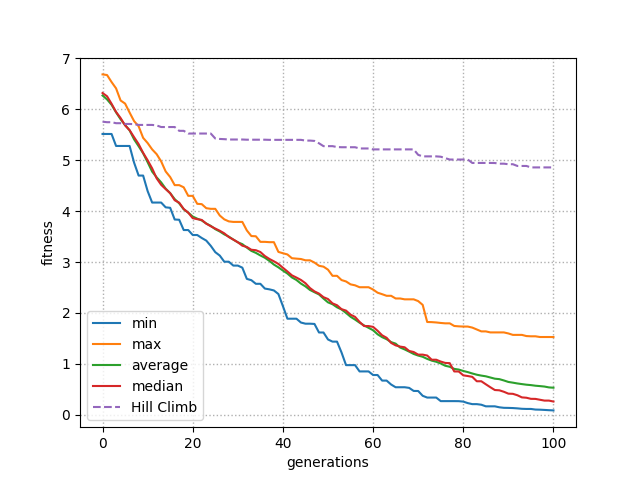
\includegraphics[width=\linewidth]{figures/es_ackley20.png}
        \caption{Resultados Ackley 20 dimensiones}
    \end{subfigure}
    \begin{subfigure}[htpb!]{1\linewidth}
        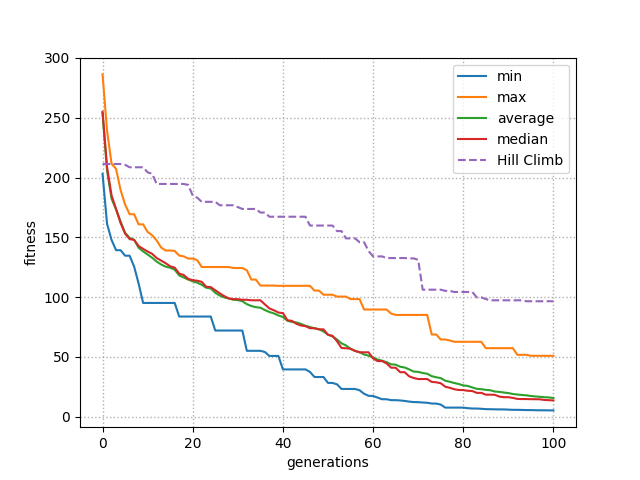
\includegraphics[width=\linewidth]{figures/es_rastrigin20.png}
        \caption{Resultados Rastrigin 20 dimensiones}
    \end{subfigure}
    \caption{Comparacion Estrategias Evolutivas vs Ascenso a la Colina}
    \label{figure:result_hc}
\end{figure}

\begin{figure}[htpb!]
    \centering
    \begin{subfigure}[htpb!]{1\linewidth}
        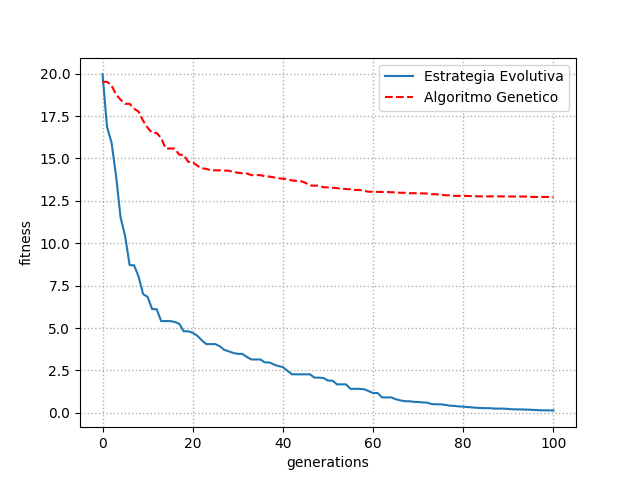
\includegraphics[width=\linewidth]{figures/ESvsGA_ackley.png}
        \caption{Resultados Ackley 20 dimensiones}
    \end{subfigure}
    \begin{subfigure}[htpb!]{1\linewidth}
        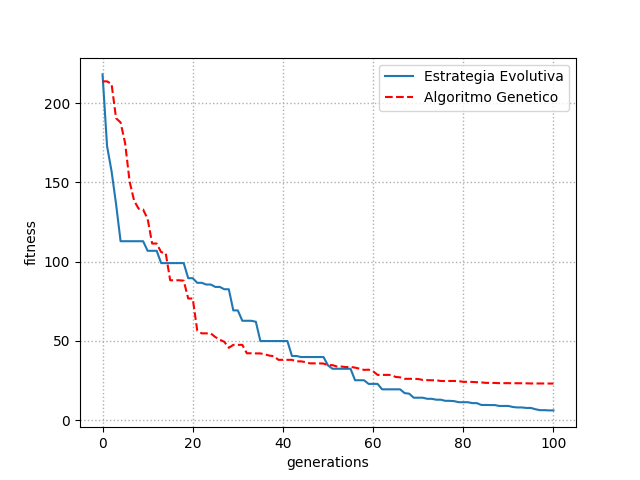
\includegraphics[width=\linewidth]{figures/ESvsGA_rastrigin.png}
        \caption{Resultados Rastrigin 20 dimensiones}
        \label{figure:esga_rastrigin}
    \end{subfigure}
    \caption{Comparacion Estrategias Evolutivas vs Algoritmo Genetico}
\end{figure}

\begin{table}[htpb!]
\centering
\begin{tabular}{|c|c|c|c|c|}
    \hline
    Problema & $\bar{x}$ & $\sigma_{\bar{x}}$ & mediana & $\sigma_{med}$ \\
    \hline
    Ackley & 0.5309 & 0.4635 & 0.2595 & 0.5394 \\
    \hline
    Rastrigin & 15.6704 & 8.9865 & 13.6117 & 9.2272 \\
    \hline
\end{tabular}
\caption{Resumen estadistico estrategia evolutiva por problema}
\label{table:result_es}
\end{table}

\begin{table}[htpb!]
    \centering
    \begin{tabular}{|c|c|c|c|c|}
        \hline
        Problema & $\bar{x}$ & $\sigma_{\bar{x}}$ & mediana & $\sigma_{med}$ \\
        \hline
        Ackley & 14.7007 & 1.1130 & 14.5960 & 1.1181 \\
        \hline
        Rastrigin & 46.1775 & 11.0827 & 44.6615 & 11.1894 \\
        \hline
    \end{tabular}
    \caption{Resumen estadistico algoritmo genético por problema}
    \label{table:results_ga}
\end{table}

\begin{table}[htpb!]
    \centering
    \begin{tabular}{|c|c|c|c|c|}
        \hline
        Problema & $\bar{x}$ & $\sigma_{\bar{x}}$ & mediana & $\sigma_{med}$ \\
        \hline
        Ackley & 5.5825 & 0.2710 & 5.6181  & 0.2734 \\
        \hline
        Rastrigin & 164.2695 & 20.6900 & 168.8914 & 21.2173 \\
        \hline
    \end{tabular}
    \caption{Resumen estadistico ascenso a la colina por problema}
    \label{table:results_hc}
\end{table}

\section{Conclusiones}

Al realizar el análisis de los datos, se puede ver en la grafica 1
existe una amplia diferencia entre las soluciones aportadas por los algoritmos.
Esto solo se refuerza al comparar los estadisticos en la tabla I y
III. \\

Respecto al algoritmo genético, se puede ver que en ocasiones este puede ser mejor que la
estrategia evolutiva como el la grafica 2.b, sin embargo en la misma 
grafica se puede comprobar que en un largo plazo es esta ultima quien consigue mejores resultados.
Nuevamente esto se puede apreciar al comparar las tablas I y
II. \\

Con esto, la estragia evolutiva demuestra ser mejor que los otros algoritmos cuando se trata de 
problemas con números reales en espacios multidimensionales, demostrando ser una de las tecnicas
mas solidas en este proposito dentro de los algoritmos evolutivos.

\begin{thebibliography}{X}
    \item Back, Hoffmeister, Schwefel. A survey of Evolution strategies.
\end{thebibliography}

\end{document}